\section{Automatic Differentiation} \label{sec:ad}
    Tracing can be very useful in many applications, such as Automatic Differentiation (AD).
    In Section \ref{sec:bg_ad} we discussed how taping is often used for both input-dependent and input-agnostic AD.
    Input-agnostic AD is especially useful for programs with little control-flow, or programs that we need the derivative of multiple inputs for.
    However, for programs with more complex control-flow, or programs that require us to only find the derivative once, input-dependent AD may be more efficient.

    If we think of the tape, a list of actions performed, as a trace, we see that tracing and AD are closely related.
    After all, we concluded in Section \ref{sec:tracing}, that our trace is a list of ``steps taken by the program run on the input'', which is very similar to the definition of a Wengert list or tape.
    We can perform forward-mode AD on a trace as is, and by recording intermediate values we make reverse-mode AD possible as well.
    In the rest of this section, we will explore exactly how we can extend tracing to perform reverse-mode AD.

    As a quick reminder, when performing reverse-AD we need to store intermediate values as they will be needed for calculating partial derivatives.
    In forward-mode AD, we often track these intermediate values as we calculate the regular answer as well as the AD answer simultaneously.
    However, in reverse-mode we will need to find these intermediate values on the forward pass, to use them for calculations on the reverse pass.
    Consider our trace from Listing \ref{lst:traced}, as a list of tuples consisting of strings as identifiers and a data constructor denoting the action taken.
    We could just add intermediate values to this structure, but we will soon find this not to be quite enough.
    
    For instance, look at the computational graph in Figure \ref{fig:forward_graph} for $f(x_1,x_2)\coloneqq x_1+(x_1\times x_2)$.
    \begin{figure}[htb]
        \centering
        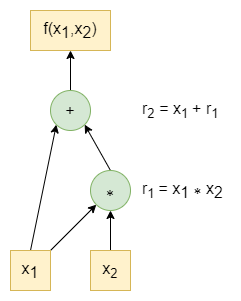
\includegraphics[scale=0.5]{diagrams/forward_example.png}
        \caption{Computational graph of $f(x_1,x_2)\coloneqq x_1+(x_1\times x_2)$}
        \label{fig:forward_graph}
    \end{figure}
    Now, let us say $x_1=5$, and $x_2=3$, and trace it using the function in Section \ref{sec:tracing}, this gives us the trace as \texttt{trace\_result} in Listing \ref{lst:forward_trace}.
    This trace is very straightforward: $x_1$ and $x_2$ are assigned their values, and the multiplication is used in the addition, so it shows up first.
    \begin{haskell}[caption=DSL definition of $f$ and its trace, label=lst:forward_trace, gobble=8]
        f :: Value -> Value -> Expression
        f x1 x2 = ELet "x1" (ELift x1) (
            ELet "x2" (ELift x2) (
                EOp2 Add (ERef "x1") (
                    EOp2 Mul (ERef "x1") (ERef "x2")
                )
            ))

        trace_result :: (TValue, Trace)
        trace_result = (TReal "r2" 20.0, [
            ("x1", TLift (TReal "x1" 5.0)),
            ("x2", TLift (TReal "x2" 3.0)),
            ("r1", TOp2 Mul "x1" "x2"),
            ("r2", TOp2 Add "x1" "r1")
        ])
    \end{haskell}
    Now, let us look at the partial derivatives of $f$ in Equation \ref{eq:reverse_ex}, as we would calculate them using reverse mode.
    In Equation \ref{eq:reverse_ex2} we see which calculations we need to perform, we define the partial derivatives or ``adjoints'' of a variable $r_i$ as $\bar{r_i}$.
    We also assume here that the ``seed'' value (the value of $\bar{f}$) is one.
    \begin{equation} \label{eq:reverse_ex}
        \begin{aligned}
            \frac{\partial f}{\partial\vec{x}}&=\frac{\partial f}{\partial r_1}\frac{\partial r_1}{\partial\vec{x}}\\
            &=\left(\frac{\partial f}{\partial r_2}\frac{\partial r_2}{\partial r_1}\right)\frac{\partial r_1}{\partial\vec{x}}
        \end{aligned}
    \end{equation}
    \begin{equation} \label{eq:reverse_ex2}
        \begin{aligned}
            \bar{f}=\bar{r_2}&=1\\
            \bar{r_1}&=\bar{r_2}\times1\\
            \bar{x_2}&=\bar{r_1}\times x_1\\
            \bar{x_1}&=\bar{r_2}\times1\\
            &+\bar{r_1}\times x_2
        \end{aligned}
    \end{equation}
    With our trace and derivative operations defined, we can now look at how we would get from one to the other.
    It is important to start at the output of the program, and since the trace function we defined in Section \ref{sec:tracing} provides us with the named output, we know where to start on our reverse pass.
    In this case, that would be $r_2$.
    As the final value in the primal calculation is the output of the program, its adjoint will be equal to the adjoint of the program or the seed value.
    This is why Equation \ref{eq:reverse_ex2} posits $\bar{f}=\bar{r_2}$.

    Since we are currently working in reverse execution order, we can just use $\bar{r_2}$ to calculate $\bar{x_1a}$ and $\bar{r_1}$ directly.
    It should be reiterated that the trace does not encode any explicit information on the order of operations taken while tracing, and while we may deduce some order from the naming of the intermediate steps (e.g. $r_1$ was done before $r_2$), we should not do this programmatically.
    Luckily, we can also discover the ``ancestors'' of any step in the trace by looking at the traced operation.
    For $r_2$ the traced operation was \texttt{TOp2 Add "x1" "r1"}, so we know that for our reverse pass, we next want to look at $x_1$ and $r_1$, as their adjoints (or part of them) rely on the value of $\bar{r_2}$ (which we can also see in Equation \ref{eq:reverse_ex2}).
    For now we will gloss over how we decide which one to do first, and look at the adjoint of $r_1$ instead.
    
    We know that $\bar{r_1}$ is dependent on $\bar{r_2}$, but how exactly is defined by the operation that produced $r_2$, which in this case is addition.
    Now, addition is really simple, as the derivative of addition of two values is the addition of the derivatives of those values.
    This is why, in Equation \ref{eq:reverse_ex2}, we multiply $\bar{r_2}$ by one to get $\bar{r_1}$, the one here denotes solely $r_1$'s contribution to $r_2$.

    Again, we can see the ancestors of $r_1$ by looking at the trace, and we find $x_1$ and $x_2$.
    Let us look at $x_2$ first.
    Again, $\bar{x_2}$ is dependent on $\bar{r_1}$, which we just calculated, but rather than an addition (like $r_2$), $r_1$ is a multiplication.
    We mentioned in Section \ref{sec:bg_ad}, in Equation \ref{eq:dualnumbers}, how the derivative of a multiplication uses both the primal part and the derivative part of a number.
    To get $\bar{x_2}$ we realize (as is visible in Equation \ref{eq:reverse_ex2} as well), that we need the primal value of $x_1$.
    We mentioned before we needed the intermediate values, and this is why.
    Multiplication is not the only operation that requires a primal component, but it is a prime example.

    Now would also be a good time to quickly reflect on the difference between the tangent (from forward-mode AD) and the adjoint.
    In forward-mode AD, the operation taken to produce some variable, would influence the tangent of that variable.
    This is somewhat intuitive, $r_1$ is a multiplication, and its tangent is $\dot{r_1}=\dot{x_1}\times x_2+\dot{x_2}\times x_1$.
    However, this is not the case for reverse-mode AD.
    In reverse-mode, we see that this information gets passed on to the adjoints of the variable used by the operation, rather than the variable it produced.
    It should be clear why: the tangents denote how the variable is influenced by a change in the inputs, while an adjoint denotes how its corresponding variable influence the outputs.
    It is important to closely observe this, mainly for implementation purposes: we want to do calculation of the (part of) the adjoint before we actually arrive at that step in the trace.
    To calculate $\bar{x_2}$ we need to know what variable $x_2$ was multiplied with (namely $x_1$).
    This means that if we do not want to helplessly bounce around through our trace, looking for references (to $x_2$ for example), it would be better to calculate (the relevant part of) $\bar{x_2}$ while we still see how it is being used.\\
    This then also bring us neatly to our next conundrum: what if a variable is used multiple times.
    In the example, this goes for $x_1$, something that we have ignored until now.
    The mathematical solution is simple: the partial derivative of a variable that is used multiple times, is just a summation of the adjoints arising from those uses.
    We see this in Equation \ref{eq:reverse_ex2}, where $\bar{x_1}$ is calculated by adding the influence to $r_1$ and the influence to $r_2$ together.
    However, implementation-wise this can be a bit of a hurdle.

    As mentioned, the trace is not in any order.
    This is unlike a typical Wengert list or tape.
    While assuring some order beforehand, or doing topological sort on the computational graph described by the trace, will in large part solve this problem, it also enforces linear execution of the reverse pass.
    And while it is not something we will linger on for now, allowing for concurrency or task parallelism while calculating the derivative, might be a nice for a performance boost, and complement the inherit data-parallelism opportunities of array operations.
    So, to solve this, we want to include some form of reference counting.
    During the forward-pass we could count how many times each variable is used in the trace, since we need to store intermediate values anyways, keeping a counter for each of these variables seems like little extra work.
    Now, on the reverse pass we can check these reference counters and every time we find part of the adjoint for a variable, we decrement its associated counter.
    If a counter has not reached zero after we have decremented it, we know its adjoint is not yet complete, and we can ignore it for now.
    If it has we can add up all the parts of the adjoint and continue from there.
    Provided there is only one output to the program, we know that all reference counters will eventually reach zero, and therefor we are assured we will calculate all adjoints.
    Of course, this provision is not as clear cut as it seems.
    Currently our DSL does not really have any room for multiple outputs, and as it is functional does not support any side-effects.
    Instead, to provide multiple outputs, currently the only way is to output an array.
    Of course, if we keep arrays in the trace, an array as output would still count as a single value.
    There is a slight discrepancy between the trace and the output if we trace away arrays however: the program will still output an array, but only its individual items are able to be found in the trace.
    This is not really a big problem, since the name of these individual outputs are derived from the name of the full list, but also because it would make little sense to trace away arrays from a program that outputs an array.

    So, we find that our trace needs to be extended with two additional things in the forward pass: intermediate values and reference counters.
    We do this in Listing \ref{lst:forward}, in the data type \texttt{Forward}, we also introduce a clone of the \texttt{Traced} data type as \texttt{Forwarded}, as we need to reference the new \texttt{Forward} type in the constructors for maps and vectorized maps.
    We also replace the list structure of \texttt{Trace} with a key-value map.
    This is not strictly necessary, but allows us to more quickly access the values in the map, while also clearly communicating there is no pre-set order to the trace.
    Each value in a \texttt{Forward} map is a 3-tuple consisting of respectively: the intermediate value, the traced operation performed, and the reference counter for this variable.
    Other than the added reference counting, and saving of intermediate values, the tracing process remains the same as it was in Section \ref{sec:tracing}.

    \begin{haskell}[caption=Forward pass data structures, label=lst:forward, gobble=8]
        data Forwarded
            = FLift TValue
            | FOp0  Op0
            | FOp1  Op1       String
            | FOp2  Op2       String String
            | FMap  [Forward] String
            | FMapV Forward   String

        type Forward = Map String (TValue, Forwarded, Int)
    \end{haskell}

    \subsection{The Reverse Pass}
        As discussed, to facilitate our reverse pass we need both the reference counting and intermediate values.
        Now let us define a function \texttt{reverse}, that makes the reverse pass.
        This reverse pass should take in an object of the \texttt{Forward} type and output a map containing the adjoints.
        In Listing \ref{lst:reverse_def} we define constructors for adjoints: one for arrays, one for sparse arrays (represented by a single index and the associated value), one for real values, and a ``null'' value we can use as a placeholder.
        We also define the \texttt{Reverse} type, which will contain these adjoints, and which is returned at the end of the reverse pass.
        The \texttt{Reverse} type maps the names of each part of the calculation to a 2-tuple containing a list of contributions of other adjoints, and its own final adjoint.

        \begin{haskell}[caption=Definition of the \texttt{Reverse} type, label=lst:reverse_def, gobble=12]
            data Adjoint
                = AArray  [Float]
                | ANull
                | AReal   Float
                | ASparse Int Float

            type Reverse = Map String ([Adjoint], Adjoint)
        \end{haskell}

        With our data types defined, we can now look at the first cases of reverse AD.
        In Listing \ref{lst:reverse} we define two functions: \texttt{reverse'} which will do most of the actual reverse pass, and a wrapper function called \texttt{reverse}.
        We also define two more utility functions: \texttt{seedAncestors} provides the adjoint of a variable to its ancestors (adding to the first part of the tuple in the \texttt{Reverse} map), it is defined in Appendix \ref{app:utility}.
        The function \texttt{getAncestors} just gets the ancestors of a specified statement in the trace, it is also defined in Appendix \ref{app:utility}.

        \begin{haskell}[caption=Reverse pass function, label=lst:reverse, gobble=12]
            reverse :: Forward -> String -> Adjoint -> Reverse
            reverse t s v = reverse' t a r
                where
                    r = seedAncestors t (Map.singleton s ([], v)) s
                    a = getAncestors t s
        \end{haskell}

